\documentclass{standalone}
\usepackage{tikz}
\usetikzlibrary{patterns, positioning}
\usepackage[sfdefault]{ClearSans} %% option 'sfdefault' activates Clear Sans as the default text font
\usepackage[T1]{fontenc}

\begin{document}
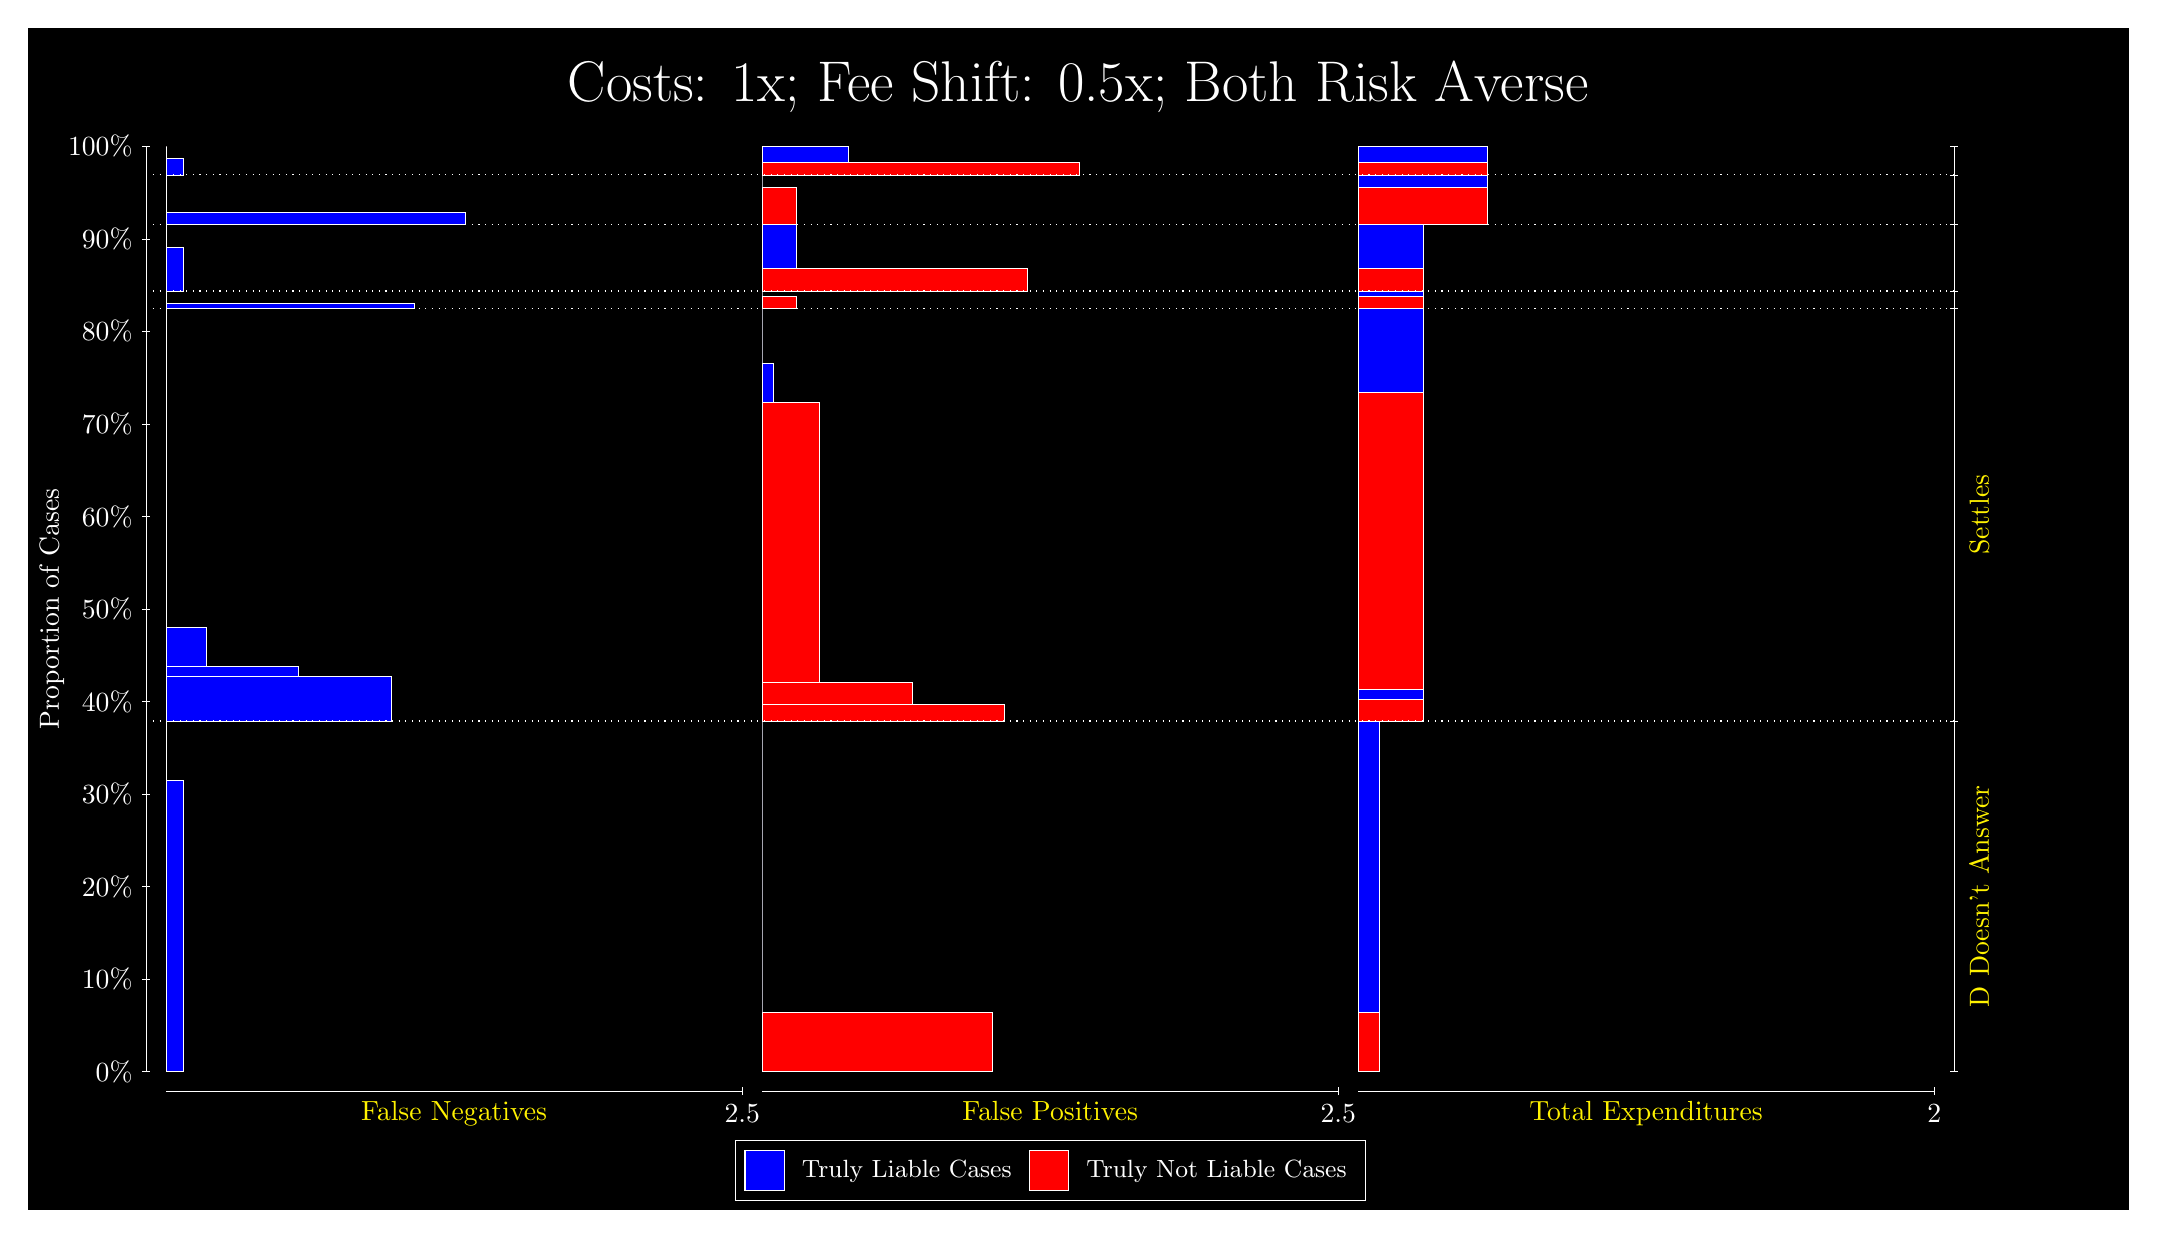
\begin{tikzpicture}
\draw[fill=black] (0,0) rectangle (26.667,15);
\draw[text=white] (0,13.5) rectangle (26.667,15) node[midway] {\huge Costs: 1x; Fee Shift: 0.5x; Both Risk Averse};
\draw[white, very thin] (1.5,1.75) -- (1.5,13.5);
\node[rotate=90, text=white, anchor=center] at (0.3, 7.625) {Proportion of Cases};
\draw[white, very thin] (1.45,1.75) -- (1.55,1.75);
\node[text=white, anchor=east] at (1.45, 1.75) {0\%};
\draw[white, very thin] (1.45,2.925) -- (1.55,2.925);
\node[text=white, anchor=east] at (1.45, 2.925) {10\%};
\draw[white, very thin] (1.45,4.1) -- (1.55,4.1);
\node[text=white, anchor=east] at (1.45, 4.1) {20\%};
\draw[white, very thin] (1.45,5.275) -- (1.55,5.275);
\node[text=white, anchor=east] at (1.45, 5.275) {30\%};
\draw[white, very thin] (1.45,6.45) -- (1.55,6.45);
\node[text=white, anchor=east] at (1.45, 6.45) {40\%};
\draw[white, very thin] (1.45,7.625) -- (1.55,7.625);
\node[text=white, anchor=east] at (1.45, 7.625) {50\%};
\draw[white, very thin] (1.45,8.8) -- (1.55,8.8);
\node[text=white, anchor=east] at (1.45, 8.8) {60\%};
\draw[white, very thin] (1.45,9.975) -- (1.55,9.975);
\node[text=white, anchor=east] at (1.45, 9.975) {70\%};
\draw[white, very thin] (1.45,11.15) -- (1.55,11.15);
\node[text=white, anchor=east] at (1.45, 11.15) {80\%};
\draw[white, very thin] (1.45,12.325) -- (1.55,12.325);
\node[text=white, anchor=east] at (1.45, 12.325) {90\%};
\draw[white, very thin] (1.45,13.5) -- (1.55,13.5);
\node[text=white, anchor=east] at (1.45, 13.5) {100\%};

\draw[white, very thin] (24.457,1.75) -- (24.457,13.5);
\draw[white, very thin] (24.407,1.75) -- (24.507,1.75);
\node[anchor=west] at (24.407, 1.75) {};
\draw[white, very thin] (24.407,6.2019) -- (24.507,6.2019);
\node[anchor=west] at (24.407, 6.2019) {};
\draw[white, very thin] (24.407,11.446) -- (24.507,11.446);
\node[anchor=west] at (24.407, 11.446) {};
\draw[white, very thin] (24.407,11.663) -- (24.507,11.663);
\node[anchor=west] at (24.407, 11.663) {};
\draw[white, very thin] (24.407,12.508) -- (24.507,12.508);
\node[anchor=west] at (24.407, 12.508) {};
\draw[white, very thin] (24.407,13.137) -- (24.507,13.137);
\node[anchor=west] at (24.407, 13.137) {};
\draw[white, very thin] (24.407,13.5) -- (24.507,13.5);
\node[anchor=west] at (24.407, 13.5) {};

\draw[white, very thin, fill=blue] (1.75,1.75) rectangle (1.9696,5.4491);
\draw[white, very thin, fill=red] (1.75,5.4491) rectangle (1.75,6.2019);
\draw[white, very thin, fill=blue] (1.75,6.2019) rectangle (4.6044,6.7759);
\draw[white, very thin, fill=blue] (1.75,6.7759) rectangle (3.4333,6.8995);
\draw[white, very thin, fill=blue] (1.75,6.8995) rectangle (2.2623,7.3928);
\draw[white, very thin, fill=red] (1.75,7.3928) rectangle (1.75,11.446);
\draw[white, very thin, fill=blue] (1.75,11.446) rectangle (4.8971,11.512);
\draw[white, very thin, fill=red] (1.75,11.512) rectangle (1.75,11.663);
\draw[white, very thin, fill=blue] (1.75,11.663) rectangle (1.9696,12.218);
\draw[white, very thin, fill=red] (1.75,12.218) rectangle (1.75,12.508);
\draw[white, very thin, fill=blue] (1.75,12.508) rectangle (5.5558,12.666);
\draw[white, very thin, fill=red] (1.75,12.666) rectangle (1.75,13.137);
\draw[white, very thin, fill=blue] (1.75,13.137) rectangle (1.9696,13.343);
\draw[white, very thin, fill=red] (1.75,13.343) rectangle (1.75,13.5);
\draw[white, very thin, fill=red] (9.3189,1.75) rectangle (12.246,2.5028);
\draw[white, very thin, fill=blue] (9.3189,2.5028) rectangle (9.3189,6.2019);
\draw[white, very thin, fill=red] (9.3189,6.2019) rectangle (12.393,6.4165);
\draw[white, very thin, fill=red] (9.3189,6.4165) rectangle (11.222,6.6951);
\draw[white, very thin, fill=red] (9.3189,6.6951) rectangle (10.051,10.255);
\draw[white, very thin, fill=blue] (9.3189,10.255) rectangle (9.4652,10.749);
\draw[white, very thin, fill=blue] (9.3189,10.749) rectangle (9.3189,11.446);
\draw[white, very thin, fill=red] (9.3189,11.446) rectangle (9.758,11.597);
\draw[white, very thin, fill=blue] (9.3189,11.597) rectangle (9.3189,11.663);
\draw[white, very thin, fill=red] (9.3189,11.663) rectangle (12.686,11.953);
\draw[white, very thin, fill=blue] (9.3189,11.953) rectangle (9.758,12.508);
\draw[white, very thin, fill=red] (9.3189,12.508) rectangle (9.758,12.98);
\draw[white, very thin, fill=blue] (9.3189,12.98) rectangle (9.3189,13.137);
\draw[white, very thin, fill=red] (9.3189,13.137) rectangle (13.344,13.294);
\draw[white, very thin, fill=blue] (9.3189,13.294) rectangle (10.417,13.5);
\draw[white, very thin, fill=red] (16.888,1.75) rectangle (17.162,2.5028);
\draw[white, very thin, fill=blue] (16.888,2.5028) rectangle (17.162,6.2019);
\draw[white, very thin, fill=red] (16.888,6.2019) rectangle (17.711,6.4804);
\draw[white, very thin, fill=blue] (16.888,6.4804) rectangle (17.711,6.6041);
\draw[white, very thin, fill=red] (16.888,6.6041) rectangle (17.711,10.379);
\draw[white, very thin, fill=blue] (16.888,10.379) rectangle (17.711,11.446);
\draw[white, very thin, fill=red] (16.888,11.446) rectangle (17.711,11.597);
\draw[white, very thin, fill=blue] (16.888,11.597) rectangle (17.711,11.663);
\draw[white, very thin, fill=red] (16.888,11.663) rectangle (17.711,11.953);
\draw[white, very thin, fill=blue] (16.888,11.953) rectangle (17.711,12.508);
\draw[white, very thin, fill=red] (16.888,12.508) rectangle (18.534,12.98);
\draw[white, very thin, fill=blue] (16.888,12.98) rectangle (18.534,13.137);
\draw[white, very thin, fill=red] (16.888,13.137) rectangle (18.534,13.294);
\draw[white, very thin, fill=blue] (16.888,13.294) rectangle (18.534,13.5);
\draw[white, dotted] (1.5,6.2019) -- (24.457,6.2019);
\draw[white, dotted] (1.5,11.446) -- (24.457,11.446);
\draw[white, dotted] (1.5,11.663) -- (24.457,11.663);
\draw[white, dotted] (1.5,12.508) -- (24.457,12.508);
\draw[white, dotted] (1.5,13.137) -- (24.457,13.137);
\draw[white, very thin] (1.75,1.5) -- (9.0689,1.5);
\node[text=yellow, anchor=north] at (5.4094, 1.5) {False Negatives};
\draw[white, very thin] (9.0689,1.45) -- (9.0689,1.55);
\node[text=white, anchor=north] at (9.0689, 1.45) {2.5};

\draw[white, very thin] (9.3189,1.5) -- (16.638,1.5);
\node[text=yellow, anchor=north] at (12.978, 1.5) {False Positives};
\draw[white, very thin] (16.638,1.45) -- (16.638,1.55);
\node[text=white, anchor=north] at (16.638, 1.45) {2.5};

\draw[white, very thin] (16.888,1.5) -- (24.207,1.5);
\node[text=yellow, anchor=north] at (20.547, 1.5) {Total Expenditures};
\draw[white, very thin] (24.207,1.45) -- (24.207,1.55);
\node[text=white, anchor=north] at (24.207, 1.45) {2};

\node[text=yellow, centered, rotate=90] at (24.777, 3.9759) {D Doesn't Answer};
\node[text=yellow, centered, rotate=90] at (24.777, 8.824) {Settles};





\draw (12.978300999999998,1.5) node[draw=none] (baseCoordinate) {};
\begin{scope}[align=center]
        \matrix[scale=0.5, draw=white, below=0.5cm of baseCoordinate, nodes={draw}, column sep=0.1cm]{
            \node[rectangle, draw, minimum width=0.5cm, minimum height=0.5cm, fill=blue] {}; &
            \node[draw=none, font=\small, text=white] (B) {Truly Liable Cases}; &
            \node[rectangle, draw, minimum width=0.5cm, minimum height=0.5cm, fill=red] {}; &
            \node[draw=none, font=\small, text=white] (B) {Truly Not Liable Cases}; \\
            };
\end{scope}

\end{tikzpicture}
\end{document}